% ============================================================================
%  3.3 DISEÑO DE LA INTERFAZ
% ============================================================================

\section{Dise\~no de la interfaz}

\subsection{Principios de dise\~no}

La interfaz del m\'odulo de inscripci\'on sigue los principios de
dise\~no establecidos en el proyecto:

\begin{itemize}
  \item \textbf{Consistencia visual:} Se reutiliz\'o el sistema de
    colores existente (\texttt{colors.ts}), el espaciado
    (\texttt{spacing.ts}) y la tipograf\'ia (\texttt{fontSize},
    \texttt{fontWeight}).
  \item \textbf{Coherencia con la app:} Los botones de inscripci\'on
    siguen el mismo estilo que el bot\'on de favoritos.
  \item \textbf{Retroalimentaci\'on visual:} El bot\'on cambia de
    apariencia al inscribirse/cancelar.
  \item \textbf{Accesibilidad:} Iconos descriptivos (Ionicons) y
    contraste adecuado.
\end{itemize}

\subsection{Pantallas del m\'odulo}

El m\'odulo se integra en dos pantallas existentes:

\subsubsection*{1. Detalle del escenario (secci\'on de eventos)}

Cada tarjeta de evento en la pantalla de detalle ahora incluye:

\begin{itemize}
  \item Nombre, fecha y hora del evento
  \item Descripci\'on (si existe)
  \item Conteo de inscritos (ej: ``3 inscritos'')
  \item Bot\'on de inscripci\'on/desinscripci\'on
\end{itemize}

\begin{figure}[H]
\centering
\figuraAPA{fig:diseno-evento-detalle}{Dise\~no de la tarjeta de evento con bot\'on de inscripci\'on}{%
  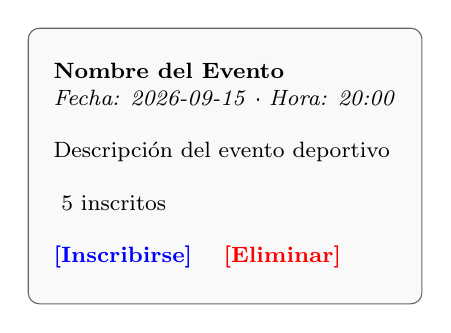
\begin{tikzpicture}[
    box/.style={rectangle, draw=black!60, rounded corners,
      minimum width=5cm, minimum height=3.5cm, align=left,
      font=\footnotesize, fill=gray!5, inner sep=8pt}
  ]
    \node[box] {
      \textbf{Nombre del Evento} \\
      \textit{Fecha: 2026-09-15 · Hora: 20:00} \\
      \\
      Descripci\'on del evento deportivo \\
      \\
      \textcolor{green!60!black}{\checkmark} 5 inscritos \\
      \\
      \textcolor{blue}{\textbf{[Inscribirse]}} \quad
      \textcolor{red}{\textbf{[Eliminar]}}
    };
  \end{tikzpicture}
}{Elaboraci\'on propia (dise\~no del componente).}
\end{figure}

\subsubsection*{2. Perfil del usuario (secci\'on ``Mis inscripciones'')}

En la pantalla de perfil se agreg\'o una nueva secci\'on que muestra
todas las inscripciones activas del usuario:

\begin{itemize}
  \item Icono de confirmaci\'on (checkmark verde)
  \item Fecha de inscripci\'on
  \item Estado vac\'io cuando no hay inscripciones
\end{itemize}

\begin{figure}[H]
\centering
\figuraAPA{fig:diseno-perfil-inscripciones}{Secci\'on ``Mis inscripciones'' en el perfil}{%
  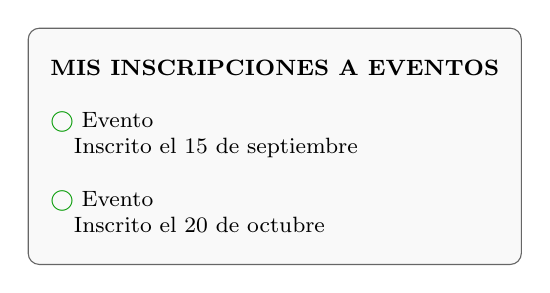
\begin{tikzpicture}[
    box/.style={rectangle, draw=black!60, rounded corners,
      minimum width=5cm, minimum height=3cm, align=left,
      font=\footnotesize, fill=gray!5, inner sep=8pt}
  ]
    \node[box] {
      \textbf{MIS INSCRIPCIONES A EVENTOS} \\
      \\
      \textcolor{green!60!black}{$\bigcirc$} Evento \\
      \quad Inscrito el 15 de septiembre \\
      \\
      \textcolor{green!60!black}{$\bigcirc$} Evento \\
      \quad Inscrito el 20 de octubre
    };
  \end{tikzpicture}
}{Elaboraci\'on propia (dise\~no del componente).}
\end{figure}

\subsection{Estados visuales del bot\'on}

El bot\'on de inscripci\'on tiene tres estados:

\begin{table}[H]
\centering
\begin{tabular}{@{}lll@{}}
\toprule
\textbf{Estado} & \textbf{Apariencia} & \textbf{Comportamiento} \\
\midrule
No inscrito & Borde azul, fondo blanco & Al tocar, inscribe \\
Inscrito & Fondo azul, texto blanco & Al tocar, pide confirmaci\'on \\
Cargando & Indicador de progreso & Deshabilitado \\
\bottomrule
\end{tabular}
\caption{Estados del bot\'on de inscripci\'on}
\end{table}
